\chapter{Style feature analysis}

\chapterquote{``Data! data! data!'' he cried impatiently. ``I can't make bricks without clay.''}{The adventure of the Copper Beeches\\Arthur Conan Doyle (1892)}

Of all the style markers used, our goal is to determine which ones vary and differ depending on the recipient of the message. With this in mind, in this chapter we are going to analyse the resulting values of measuring each message with the previously explained system.

The first step in our analysis is to prepare the data. We have to categorise the different contacts depending on its relationship with the sender, choose the features that we are going to study and modify its values in order to have the data ready for being analysed. All of this is explained in Section \ref{sect:DatPrep}.

\section{Data preparation}\label{sect:DatPrep}
First of all it is necessary to classify the different recipients of the analysed messages. For this purpose, all the contacts (a total of 337 different e-mail addresses) have been divided into twelve categories depending on their relationship with the analysed user. These categories are: \textit{friend}, \textit{acquaintance}, \textit{company} (in this category are grouped all the company contacts with which the user has had a relationship to contract their service), \textit{university}, \textit{boss}, \textit{colleague}, \textit{professor}, \textit{relative}, \textit{stranger}, \textit{university position}, \textit{casting} (the people with which the user was in touch in order to manage a theatre casting belong to this relationship type) and \textit{company recruiting} (where are classified the e-mail addresses that the user contacted to be a candidate in a recruiting process).

Our style markers were applied to each message, so it is necessary to categorise the different e-mails. With this in mind, we determine the category of the message depending on its recipient(s). Classifying e-mails destined for a single e-mail account is a trivial problem (its category will be the one assigned to the message's recipient). We can also directly classify those messages whose recipients all belong to the same category. E-mails that have several receivers from different categories are automatically classified when they have only one addressee in the recipients field \textit{To} (they are grouped in that contact's category), which represents the main recipient(s) of the message, while the \textit{Cc} (Carbon Copy) and \textit{Bcc} (Blind Carbon Copy) fields have the purpose of keeping the addressees in there informed. Otherwise, we classify it one by one (there were only 14 messages out of 921 that we had to review) depending on the type of relationship we think indicates the wording of the message.

After this classification process, we obtained the distribution of relationship categories that we can see in Figure \ref{fig:distr}. As we can observe, we have not equally distributed classes and this represent a problem in our data analysis. Indeed, the biggest class (the \textit{professor} class) represents approximately $39.41$\% of the total, while the second one (\textit{university position}) in size is the $13.25$\%. And, of course, both categories are far from the smallest class (\textit{acquaintance}) which only represents approximately $0.33$\%. Despite this unbalanced distribution between the different categories, we will analyse this data set and obtain conclusions in order to detect the most significant features for differentiating the writing style based on the recipient of the e-mail. We have to take into account that the conclusions will be closely linked to the data obtained given the small sample size.

\begin{figure}
	\centering%
	\centerline{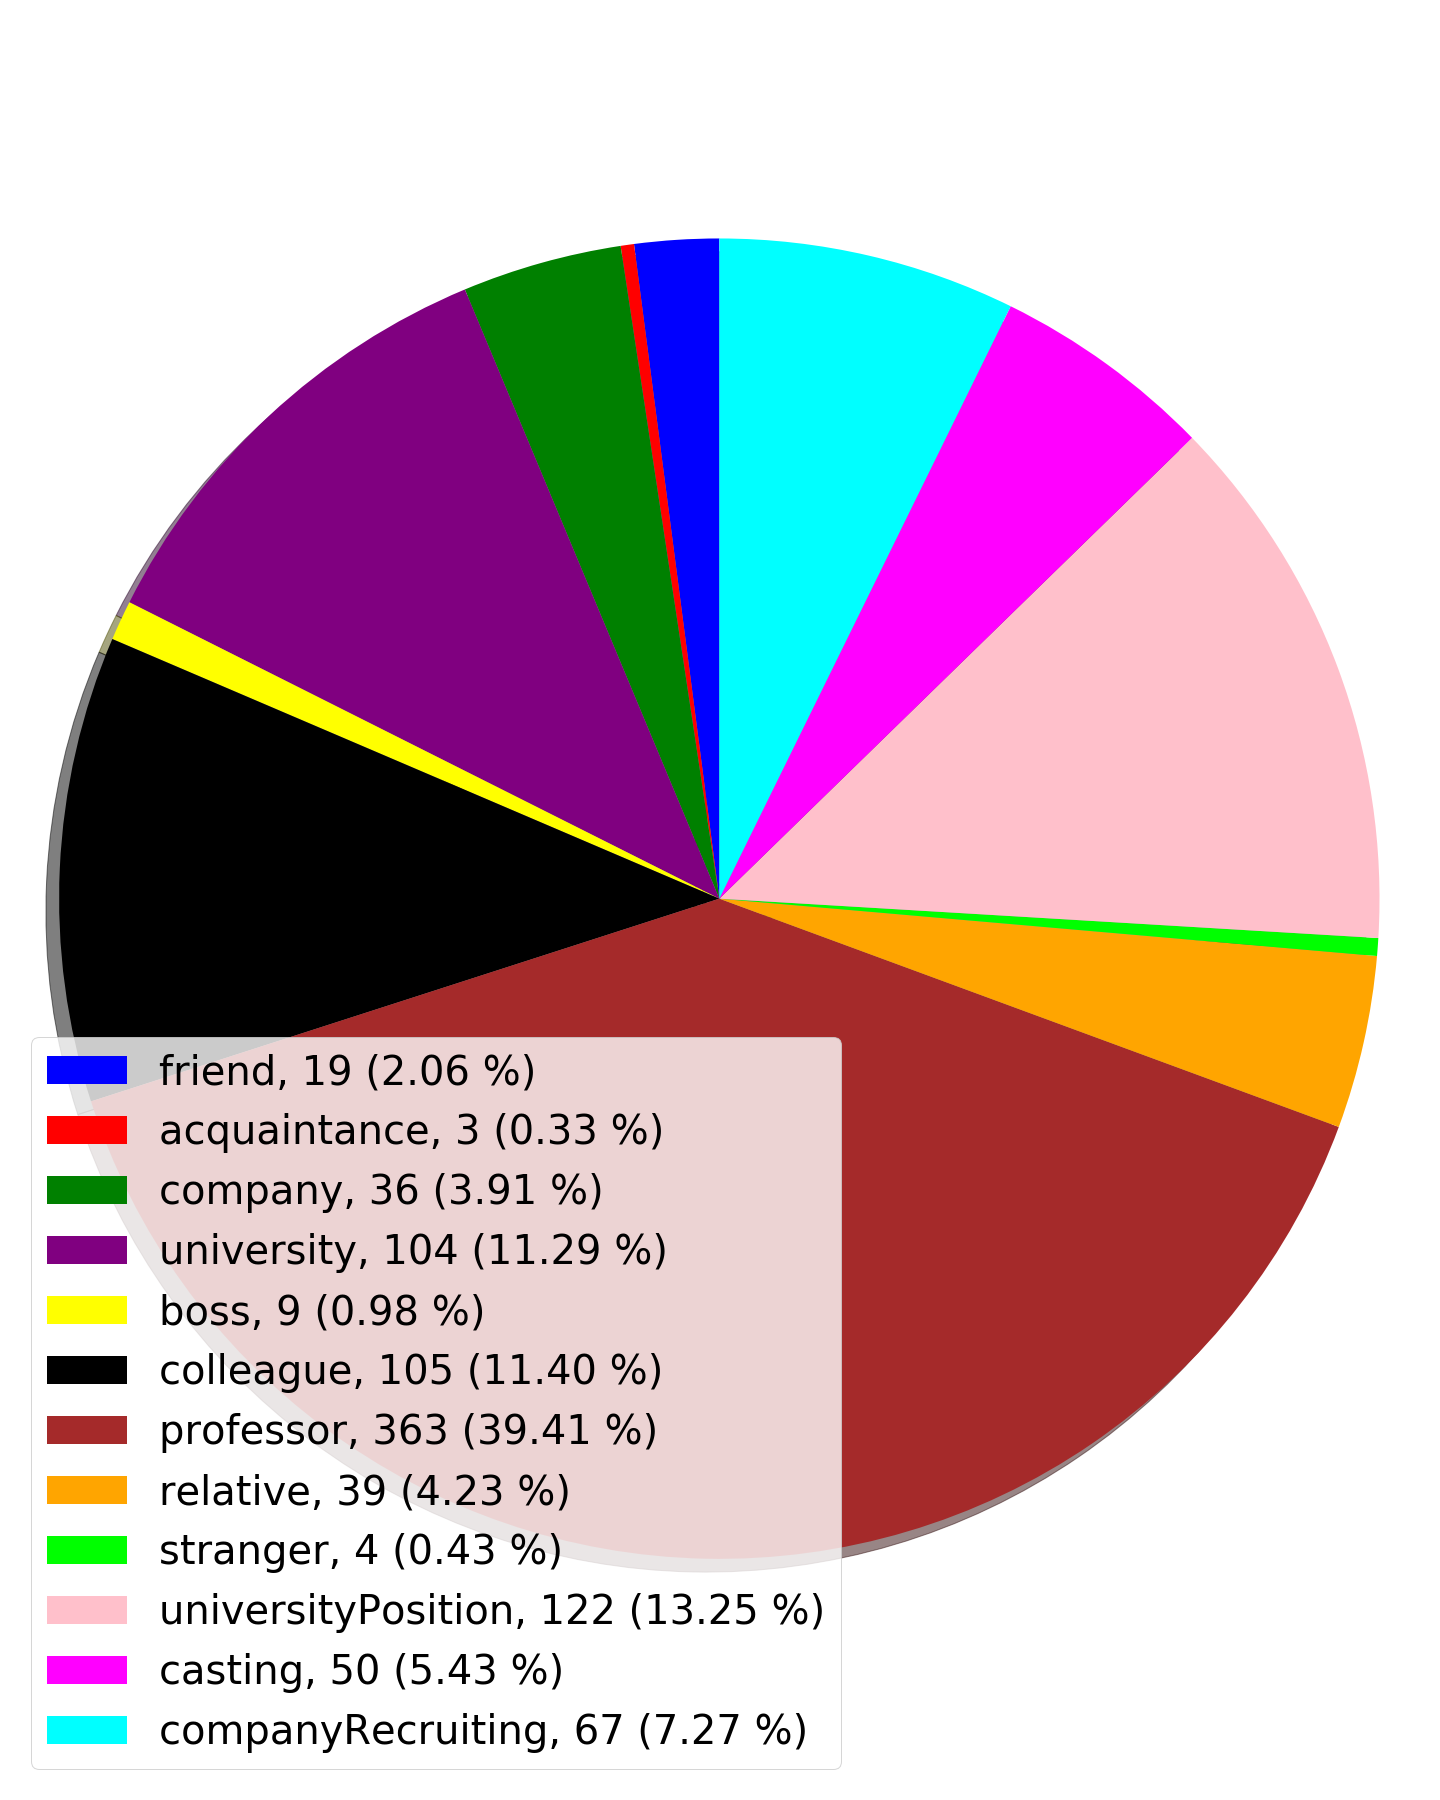
\includegraphics[width=0.5\textwidth]{Imagenes/Bitmap/classdistributionpie.png}}%
	\caption{Distribution of relationship categories}%
	\label{fig:distr}
\end{figure}

Once all e-mails are classified in our twelve categories, we have to choose which style features we are going to analyse. At first glance, there are features of each message (the attributes of the \textit{Metrics} class, which can be looked up in Section \ref{section:measmod}) from which we are not be able to extract significant numerical information, such as the sender of the e-mails (which is the same for all of them), the subject and the identifier of the thread they belong to (called \textit{threadId}). Besides, as the distribution of the different categories is too unbalanced, we risk losing underrepresented classes if a time-related weight is applied over the several metrics. For this reason, we decide not to take the date into account for our analysis.

\begin{figure}[p]
	\centering%
	\centerline{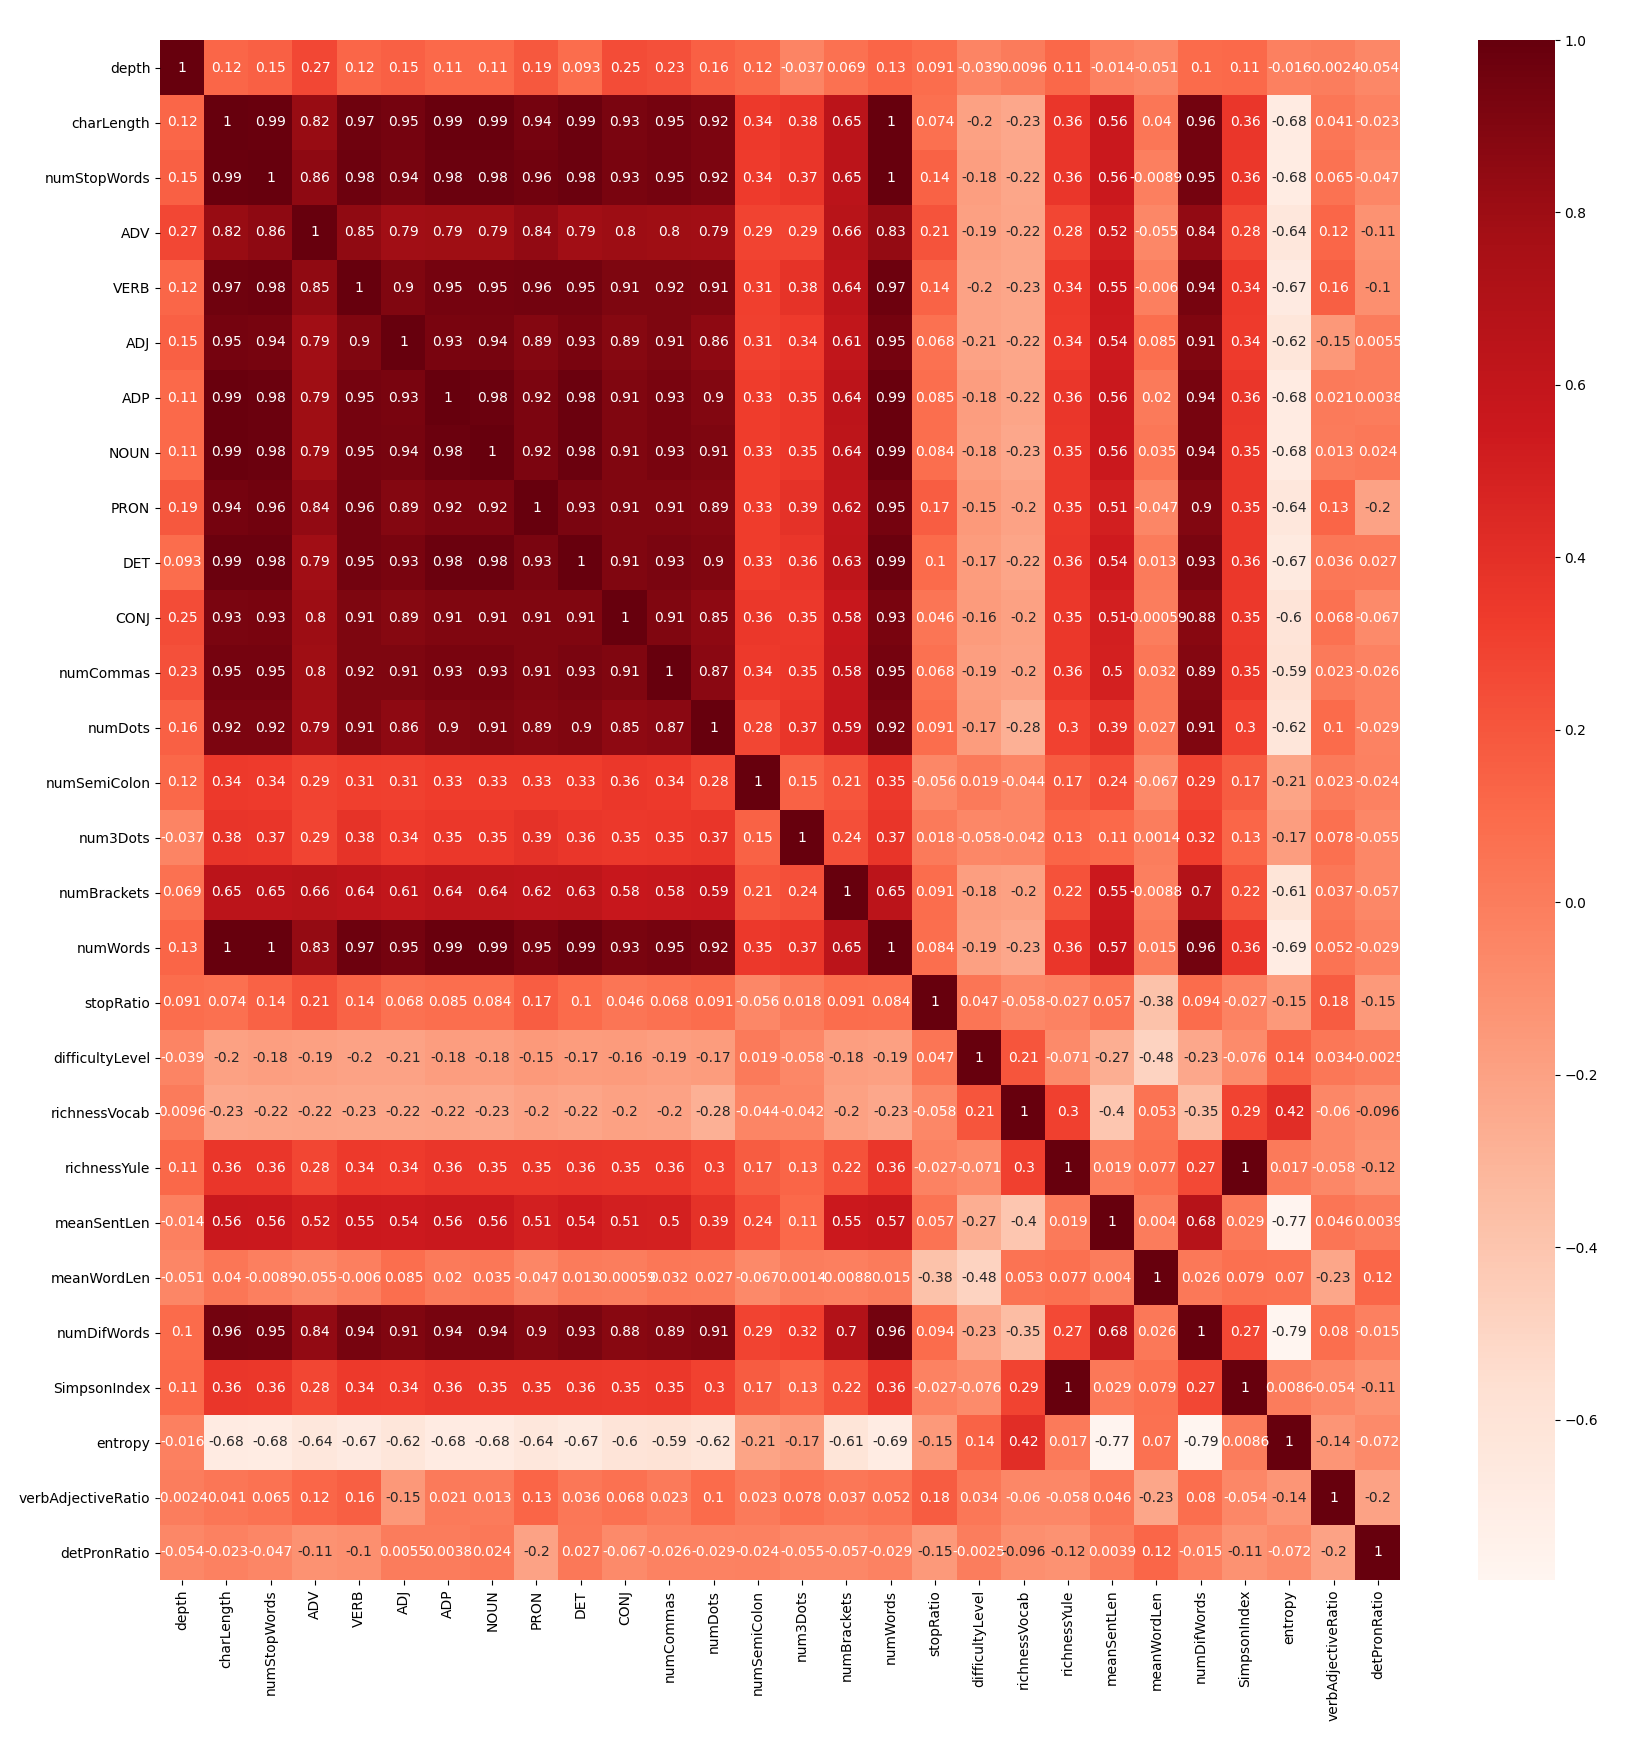
\includegraphics[width=0.98\paperwidth]{Imagenes/Bitmap/correlationmatrix.png}}%
	\caption{Pearson correlation coefficient between each pair of features}%
	\label{fig:correlation}
\end{figure}

In addition to the mentioned features, we have removed from our data set the following writing style markers: \textit{metricsSentences}, \textit{wordLength}, \textit{sentLength}, \textit{sentNumWords} and \textit{wordsAppearance}. All of them describe a distribution of a style feature (or several as the \textit{metricsSentence} attribute) through a dictionary or list structure, which are excessively complex to manipulate with the rest of the style features using common machine learning techniques. Furthermore, they would produce a big amount of NaN (Not a Number) values in our data set, because of the diversity in the number of sentences and words used in each e-mail (for instance if a message has an only sentence, all the style metrics related to the subsequent sentences will have a NaN value).

Therefore, we are going to work with 27 writing style markers, the depth of the message (perhaps we can find significant conclusions with this parameter) and the identifier of each message as index of each of the rows of our data set.

E-mail messages, by nature, do not contain a constant number of words from message to message. To overcome this variable and now that we have decided the style characteristics that we are going to study, the features are normalized, because techniques that require it (such as the K-Means algorithm) are used. Besides, we are going to find some NaN values, for example in \textit{verbAdjectiveRatio} and \textit{detPronRatio} in the messages where there are not adjectives or pronouns, respectively. The solution to overcome this problem, due to some algorithms do not admit data set with this type of values, is to assign the value of the arithmetic mean in the sample of individuals in the category to which the message belongs of the style marker in question, when it will be necessary. In other words, if an e-mail of the category $C$ has a NaN value in the style metric $M$, it will be replaced by the value of the arithmetic mean of the feature $M$ of the rest of the messages of class $C$.

It would be desirable to be able to visualize the main descriptive statistics to get an idea of each of the metrics. Nevertheless, given the big amount of style markers, the visualization becomes very complicated. For this reason, in the following sections, we try to reduce the dimensionality of the system in order to be able to explain the main characteristics and describe the writing style.

Before starting with the data analysis, we are going to study the relationship between each selected feature. To carry it out, the Pearson correlation coefficient \citep{benesty2009pearson} is going to be calculated between each pair of style markers. It is a measure of linear dependence between two quantitative random variables. Unlike covariance, Pearson's correlation is independent of the scale of measurement of the variables. Less formally, we can define Pearson's correlation coefficient as an index that can be used to measure the degree of relationship of two variables as long as both are quantitative and continuous. It has a value between $-1$ and $+1$, where 1 is total positive linear correlation, $0$ is no linear correlation, and $-1$ is total negative linear correlation.

As a result of the calculation of the Pearson correlation coefficient, we obtain the heat map of the Figure \ref{fig:correlation}. Logically, there is a positive linear correlation between those metrics that are strongly influenced by the length of the message. These pairs of style markers represent almost all results obtained close to the value 1. Moreover, there is a total positive linear correlation between Yule's Characteristic and Simpson's Index, which was predictable given the definition of one style feature with respect to the other (see Section \ref{ssect:vocabf}). These relationship will be taken into account during the analysis of the data.

\section{Clustering}
In an initial approach, we are interested in knowing how well metrics fit our twelve category classification. To achieve this, we have executed two popular clustering algorithms which are going to group our set of elements (composed of the different style features) in such a way that members of the same group (called a cluster) are more similar in one way or another. These algorithms are K-Means \citep{hartigan1975clustering} and DBSCAN \citep{ester1996density}.

\begin{algorithm}
	\begin{algorithmic}[1]
		\REQUIRE Data set $X$ (represented as a matrix whose columns are the features and whose rows are the different samples) with missing values, number of clusters $k$ and the maximum number of iterations to perform $maxiter$.
		\ENSURE A vector $labels$ that indicates to which cluster each element belongs and a data set $X^\prime$ which is a copy of $X$ with the missing values filled in.
		\STATE $X^\prime = X$
		\STATE $missing = $ list of positions (pair of rows and columns) of the missing values of $X$
		\FOR {$(row, column)$ in $missing$}
		\STATE $X^\prime[row, column] = mean(X[, column])$
		\ENDFOR
		\STATE $i = 1$
		\STATE $converge =$ \FALSE
		\STATE $prevlabels, prevcentroids = KMeans(init = random, k, X^\prime)$
		\FOR {$(row, column)$ in $missing$}
		\STATE $X^\prime[row, column] = prevcentroids[prevlabels[row]][column]$
		\ENDFOR
		\WHILE {$i < maxiter$ $\land$ $\lnot converge$}
		\STATE $labels, centroids = KMeans(init = prevlabels, k, X^\prime)$
		\FOR {$(row, column)$ in $missing$}
		\STATE $X^\prime[row, column] = centroids[labels[row]][column]$
		\ENDFOR
		\STATE $converge =$ $(prevlabels == labels)$
		\IF{$\lnot converge$}
		\STATE $prevlabels = labels$
		\STATE $prevcentroids = centroids$
		\STATE $i = i + 1$
		\ENDIF
		\ENDWHILE
		\RETURN $labels, X^\prime$
	\end{algorithmic}
	\caption{K-Means with missing values}\label{alg:kpod}
\end{algorithm}

Both algorithms require a parameter (in the case of K-Means the parameter is the number of clusters and in the case of DBSCAN the threshold distance that determines a neighbourhood of elements) which has to be defined before their execution. To make the decision of the initial value of the parameter there are methods based on the internal and cluster dispersion obtained. For this purpose, measures are taken to help the decision, such as the Silhouette Coefficient \citep{rousseeuw1987silhouettes}. It is a method of interpretation and validation of consistency within clusters of data. The technique provides a succinct graphical representation of how well each object has been classified. The best value is 1 and the worst value is -1. Values near 0 indicate overlapping clusters. Negative values generally indicate that a sample has been assigned to the wrong cluster, as a different cluster is more similar. Likewise, we can obtain a general idea of the behaviour of the clustering by calculating the mean Silhouette Coefficient for all samples.

Furthermore, we need to assess how much our classification resembles the clusters obtained after the execution of each of the algorithms. For this evaluation, we can use the Adjusted Rand Index, which is a form of the Rand index \citep{rand1971objective} that conforms to the random grouping of elements. The Adjusted Rand index is thus ensured to have a value close to 0.0 for random labelling independently of the number of clusters and samples and exactly 1.0 when the clusterings are identical (up to a permutation).

Due to the presence of NaN values, we are not able to use the K-Means algorithm directly on the data. Instead of replacing the NaN values as we have explained in Section \ref{sect:DatPrep}, we are going to use a slight variation from the K-POD algorithm \citep{chi2016k}, which runs K-Means iteratively while it modifies the cells where the value is missing by assigning the value of the centroids. The algorithm that we are going to use, similar to the K-POD, is the one shown in Algorithm \ref{alg:kpod}, where we have two invoked functions. The first one is \textit{mean}, which returns the mean of the given array without taking into account the missing values. The second one, \textit{KMeans}, is a function that applies the K-Means algorithm given a set of initial centroids (or it will generate them randomly), the number of clusters and the dataset. It returns an array as long as the number of rows of the given dataset which indicates the cluster index (through an integer) that each element belongs to and the coordinates (features values) of the centroid of each cluster (it will be a matrix with as many rows as the number of cluster and as many columns as the numbers of features).

Now that we have chosen the algorithm, we execute it with different $k$ parameter (the number of clusters). The rest of the input will be the normalised data with the NaN values and with a maximum of 100 iteration. With each $k$-dependent execution, we will calculate the Silhouette Score (which is the mean of the Silhouette Coefficient of all samples) and the Adjusted Rand Index given the real classification. As a result of this we obtain Figures \ref{fig:nkmeanssil} and \ref{fig:nkmeansari}.

\begin{figure}
	\hspace{-1cm}\begin{minipage}[b]{0.4\paperwidth}
	\centerline{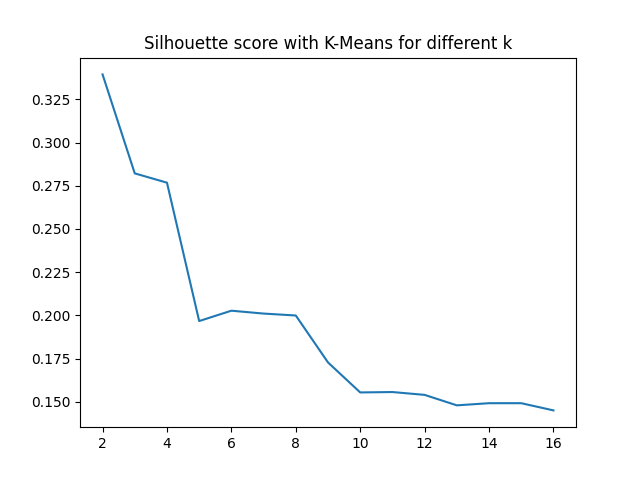
\includegraphics[width=\textwidth]{Imagenes/Bitmap/Clustering/normkmeanssil.png}}%
	\caption{Silhouette Score with K-Means for different $k$}%
	\label{fig:nkmeanssil}
	\end{minipage}
	\hspace{0.4cm}
	\begin{minipage}[b]{0.4\paperwidth}
		\centerline{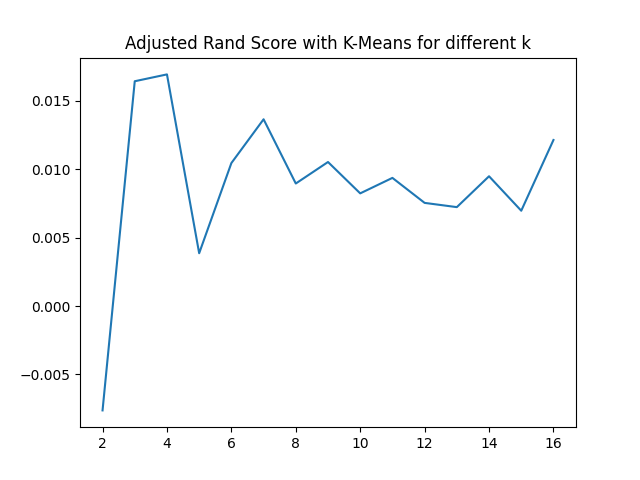
\includegraphics[width=\textwidth]{Imagenes/Bitmap/Clustering/normkmeansrand.png}}%
		\caption{Adjusted Rand Index with K-Means for different $k$}%
		\label{fig:nkmeansari}
	\end{minipage}
\end{figure}

In respect of the Silhouette Score analysis (which is shown in Figure \ref{fig:nkmeanssil}), with the given values, we are able to claim that, in general, as the number of groups increases the Silhouette Score decreases. This fact indicates us that the best number of clusters in order to achieve a good differentiation between each group of elements is two, which is not in line with our classification model. Not surprisingly, these results, which do not fit well in the established categories, are accompanied by poor values of the Adjusted Rand Index. As we can observe in Figure \ref{fig:nkmeansari}, all the obtained values with any number of cluster is very close to zero, which means, as we have previously explained, that the obtained classification does not match with ours.

In the case of DBSCAN algorithm, we are going to replace the missing values as we have explained in Section \ref{sect:DatPrep}. This clustering technique needs two different parameters: the threshold distance that determines a neighbourhood of elements (denoted by $\varepsilon$) and the minimum number of elements that forms a cluster. We will assign the value of three to this last parameter. This choice is motivated by the distribution between the different categories that we have previously defined. As we can observe in Figure \ref{fig:distr}, the smallest class has three elements in it, so it would not be consistent with our classification if a minimum number bigger than three is established. Moreover, the value of one does not make sense, since all the points of your data set will be a cluster (we would lose the possibility of detecting noise which is one of the advantages of DBSCAN over K-Means), and with 2 the result will be the same as the hierarchical cluster \citep{nielsen2016hierarchical} with the single-link metric, with the cut at the height of the dendrogram $\varepsilon$.

As we have done with K-Means, we are going to execute the DBSCAN algorithm with different $\varepsilon$ parameters. Besides, both the euclidean and manhattan metric are going to be used for this analysis. However, we will get similar results in both cases, so we are going to present the values obtained with the euclidean metric (see Figure \ref{fig:dbscaneu}).

\begin{figure}[t]
	\centering%
	\centerline{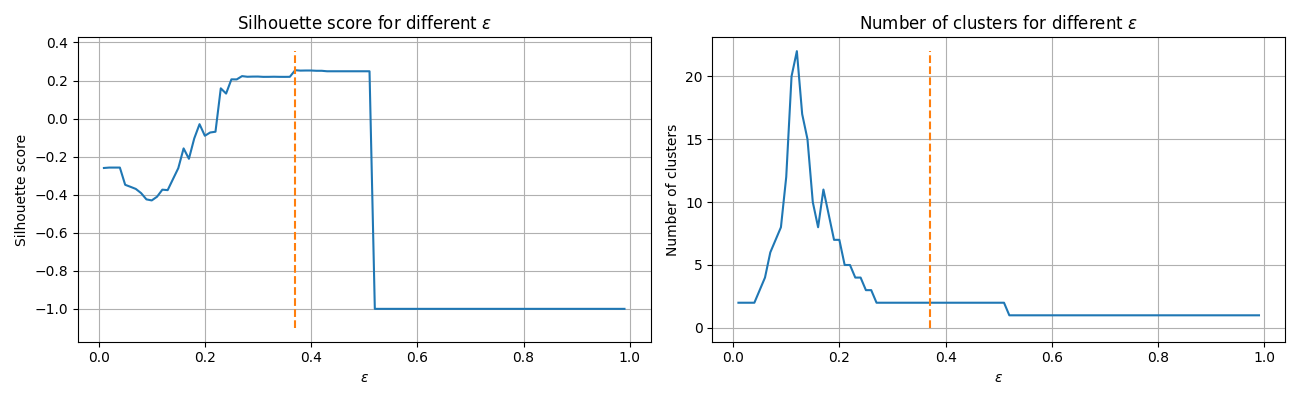
\includegraphics[width=\textwidth]{Imagenes/Bitmap/Clustering/dbscansil.png}}%
	\caption{Results of DBSCAN execution with euclidean metric}%
	\label{fig:dbscaneu}
\end{figure}

As in the case of the K-Means algorithm, we can find the maximum Silhouette Score with two clusters, which is not in line with our classification model. Furthermore, as we can see in Figure \ref{fig:dbscanari}, we find again values very close to zero in the Adjusted Rand Index analysis.

In conclusion, using the clustering techniques to classify the messages according to the selected metrics, as expected, we do not obtain significant results that fit our model or allow us to group the different e-mails in another way. One of the problems found to achieve this is the great amount of states that each element has, that is, the high number of dimensions of the system. We also find this inconvenience when we try to get the main statistics of the different features that describe the messages. Therefore, it is an issue that must be addressed (the reduction of dimensionality), especially trying that this reduction serves to adapt to the categorization carried out or to obtain a smaller number of parameters that define the writing style.

\begin{figure}[h]
	\centering%
	\centerline{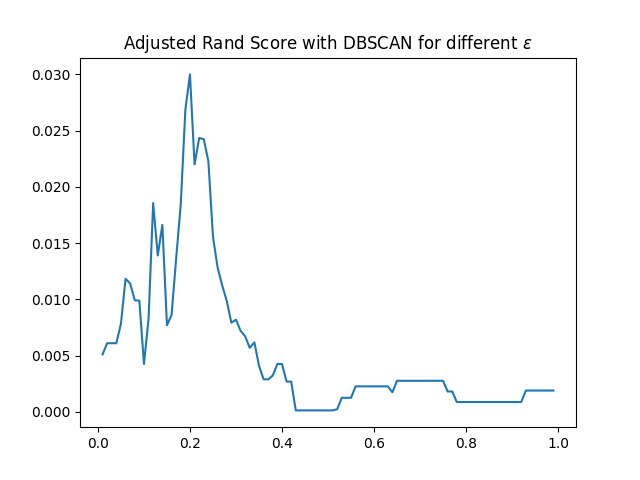
\includegraphics[width=0.5\textwidth]{Imagenes/Bitmap/Clustering/dbscanari.png}}%
	\caption{Adjusted Rand Index of DBSCAN with euclidean metric}%
	\label{fig:dbscanari}
\end{figure}